\documentclass[./bab_4.tex]{subfiles}
\begin{document}
\section{Pembahasan}
\subsection{Docker Compose}
\paragraph*{}Merujuk pada gambar \ref{isicompose} di baris
nomor pertama terdapat syntax ``version'', syntax ini
berfungsi untuk menentukan file konfigurasi docker compose
tersebut ditulis dengan menggunakan file format versi
keberapa. Versi docker compose tidak wajib tapi dianjurkan
untuk disertakan. Hal tersebut dilakukan untuk
kompatibilitas dengan versi lama.

\paragraph*{}Pada baris ke-7 di gambar \ref{isicompose}
terdapat syntax ``port''. Disini ditentukan port yang akan
dibuka ke publik. Pada nomor port yang ditentukan tersebut
terdapat dua port yang ditulis seperti berikut ``80:80''.
Nomor port sebelum titik dua (:) merupakan port milik host,
sedangkan port setelahnya merupakan milik container, jadi
port 80 milik host akan disambungkan ke port 80 milik
container. Sesuai dengan rancangan di gambar \ref{rancangan}
port 80 dan 443 dieksps sehingga dapat diakses oleh publik.

\paragraph*{}Pada baris ke-10 di gambar \ref{isicompose}
terdapat syntax ``volumes''. Syntax ini digunakan untuk
menentukan direktori atau berkas yang akan di-\textit{mount}
ke dalam kontainer. Seperti pada gambar \ref{rancangan},
direktori ``cert'' dan ``www'' di-\textit{mount} ke
kontainer ``php-apache''.

\paragraph*{}Selanjutnya pada gambar \ref{rancangan}
kontainer ``php-apache'' bergantung pada kontainer database,
oleh karena itu, pada baris nomor 13 di gambar
\ref{isicompose} terdapat syntax ``depends\_on''. Dengan
menentukan syntax tersebut maka kontainer database akan
otomatis dijalankan jika kontainer ``php-apache'' berjalan.

\paragraph*{}Kontainer database di gambar \ref{isicompose}
terdapat syntax ``environment'' di baris 21. Syntax ini
digunakan untuk menentukan variabel yang akan dipakai untuk
mengatur opsi yang ada di kontainer. Untuk opsi yang bisa
dipakai bisa merujuk ke halaman docker hub dari image docker
yang dipakai. Pada gambar \ref{rancangan}, kontainer
database memiliki port internal 3306, tetapi port tidak
ditentukan di syntax ``port''. Hal ini dikarenakan syntax
``port'' hanya diperlukan jika akan membuka port secara
publik. Sedangkan untuk port internal ditentukan di
Dockerfile. Pada image yang digunakan oleh kontainer
database, port 3306 sudah dibuka secara \textit{default}.

\subsection{LAMP}

\begin{figure}[ht!]
  \begin{center}
    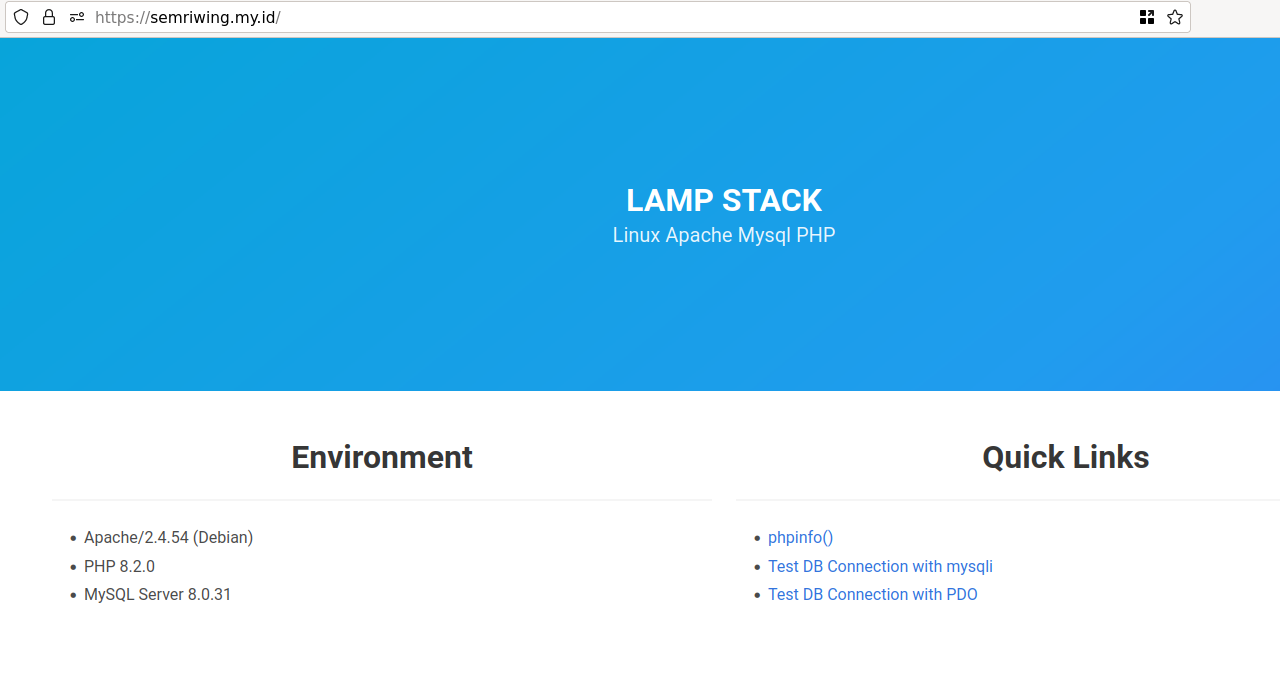
\includegraphics[width=0.95\textwidth]{halamanutama}
  \end{center}
  \caption{Halaman utama server}
  \label{halamanutama}
\end{figure}

\paragraph*{}LAMP \textit{stack} yang dipasang di server berhasil
berjalan dengan baik seperti yang dilihat pada gambar
\ref{halamanutama}. Apache dapat dengan baik menampilkan
halaman index. Untuk aplikasi yang dibuat oleh Divisi
Backend dan Divisi Frontend yang dideploy dengan
menggunakan LAMP \textit{stack} tersebut akan dilakukan
pengujian kembali.


\subsection{Halaman Login Webclient}
\begin{figure}[ht!]
  \begin{center}
    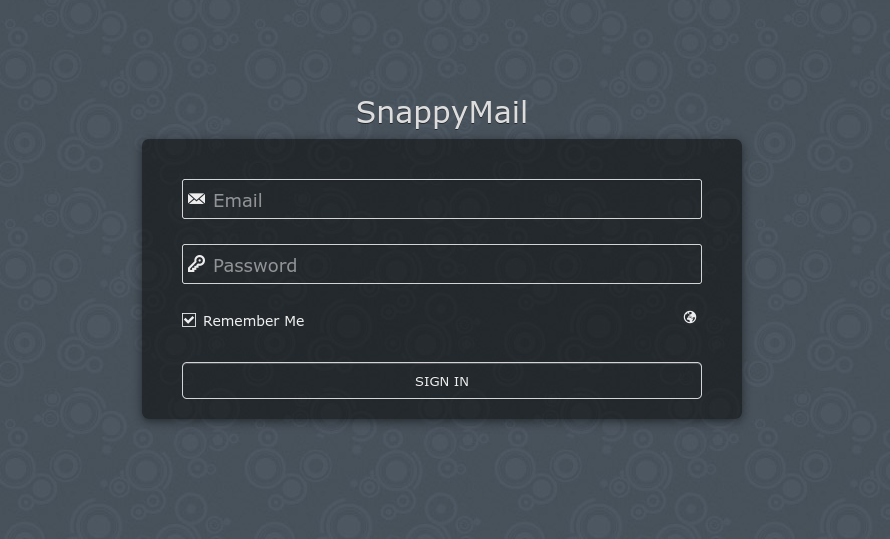
\includegraphics[width=0.95\textwidth]{login}
  \end{center}
  \caption{Halaman Login Email}
  \label{login}
\end{figure}
\paragraph*{}Gambar \ref{login} adalah tampilan halaman
login dari webmail snappymail. Pengguna dapat mengakses
langsung akun email melalui browser. Pengguna dapat
mencentang remember me, sehingga tidak perlu memasukkan
password setiap saat.

\subsection{Mengirimkan Email}
\begin{figure}[ht!]
  \begin{center}
    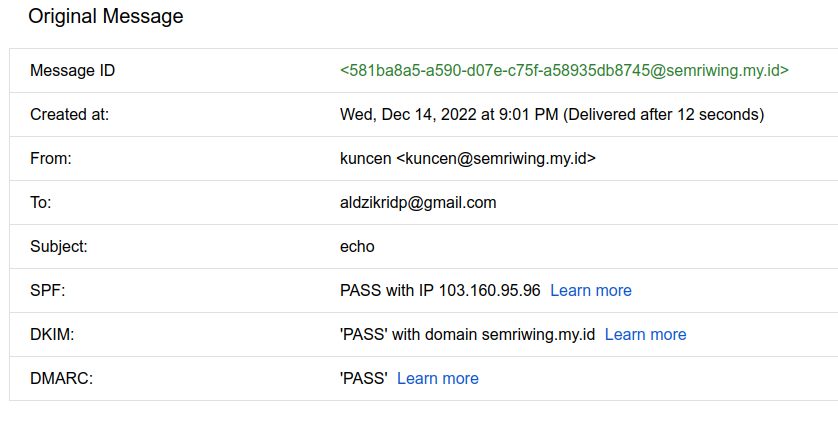
\includegraphics[width=0.95\textwidth]{gmailtest}
  \end{center}
  \caption{Email yang dikirimkan berhasil melalui cek}
  \label{gmaitest}
\end{figure}
\paragraph*{}Syarat utama untuk email server yang dibuat
adalah dapat mengirimkan email ke akun email Gmail. Hal ini
dikarenakan Gmail adalah salah satu layanan penyedia email
yang dipakai oleh banyak orang sehingga email server yang
dibuat bisa dipastikan bisa menjangkau banyak orang. Selain
itu Gmail juga menerapkan metode verifikasi email pencegah
spam secara lengkap. Oleh karena itu dengan melakukan pengujian
terhadap email Gmail, email server yang sudah dibuat bisa
dianggap sudah memenuhi standar jika berhasil masuk ke inbox
Gmail.

\paragraph*{}Pada server email yang dibangun di penelitian
ini, email yang dikirimkan oleh server ini berhasil melewati
ketiga autentikasi di atas, nampak pada gambar
\ref{gmaitest}.

\subsection{Menerima Email}
\begin{figure}[!ht]
  \begin{center}
    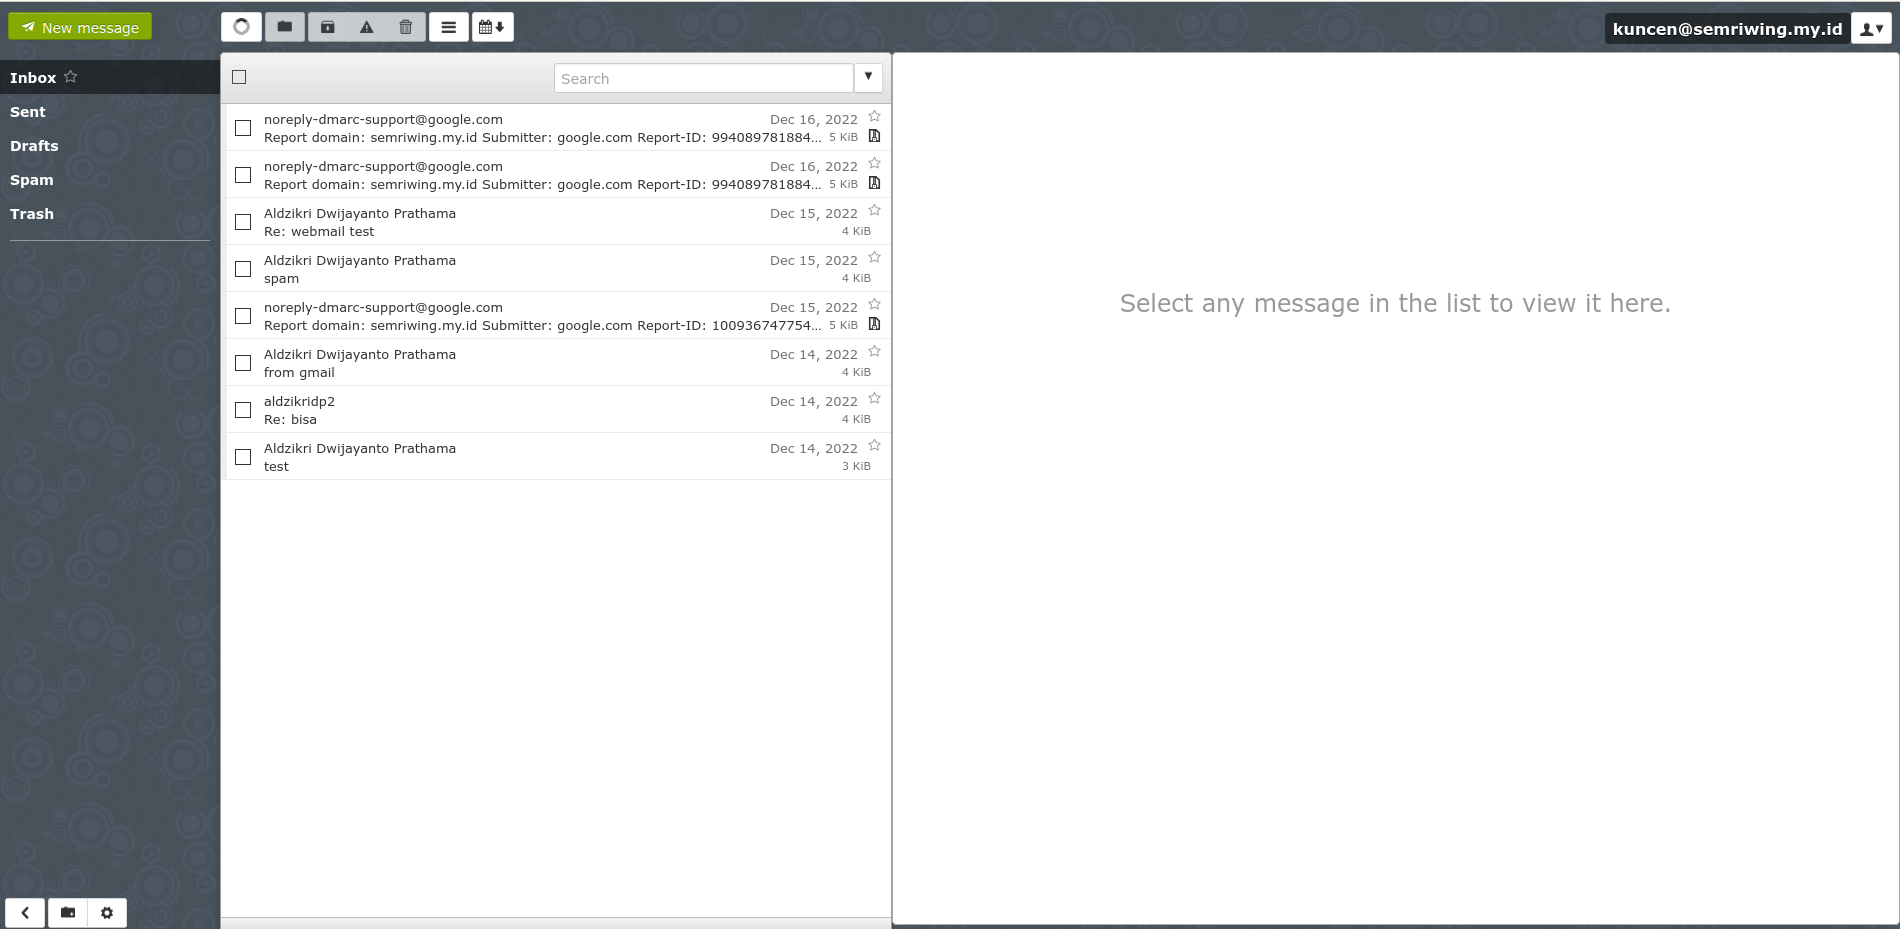
\includegraphics[width=0.95\textwidth]{inbox}
  \end{center}
  \caption{Inbox Email}
  \label{inbox}
\end{figure}
\paragraph*{}Gambar \ref{inbox} merupakan tampilan dari
inbox email server yang dibuat. Email yang dikirimkan dari
akun Gmail berhasil masuk ke email server.

\end{document}
